%!TEX root = ../main.tex
%%%%%%%%%%%%%%%%%%%%%%%%%%%%%%%%%%
% Links:
%
% Difficulty: Companies: 
%%%%%%%%%%%%%%%%%%%%%%%%%%%%%%%%%%

\chapter{Number of Dice Rolls With Target Sum}
\label{ch:dice_rolls}
\section*{Introduction}
Dices have been around for quite a long time, with the oldest dice known actually discovered in Iran
as part of Backgamonn\footnote{One of the oldest board game. A two-players game where pieces are
moved around between twenty-four triangles according to the roll of two $6$ faces dices. The goal of
each player is to remove all of their $15$ pieces before the other player.} set more than a
staggering five-thousands years old! 

We are used to the common $6$ faces dice (see Figure \ref{fig:cycle_in_list:6faces_dice}) but in
reality dices come in all shapes and forms like the $20$ faces icosahedron (see Figure
\ref{fig:dice_rolls:20faces_dice}) shape dice or the $12$ faces dodecahedron dice (see Figure
\ref{fig:dice_rolls:12faces_dice}). For this problem we will use up to $30$ dices at the same time
each with up to $30$ faces and we are going to calculate the number of ways we can obtain a certain
target value when thrown all at the same time.


\section{Problem statement}
\begin{exercise}
You have $d$ dice, and each die has $f$ faces numbered $1, 2, \ldots..., f$.

Write a function that returns the number of possible ways to roll the dices so the sum of the upper
faces equals a given number target number $t$. Because this number can be very large, the answer
should be returned modulo $10^9 + 7$.

	\begin{example}
		\hfill \\
		Given $d=1$, $f=6$ and $t=6$ the function should return $1$.
	\end{example}

	\begin{example}
		\hfill \\
		Given $d=2$, $f=6$ and $t=7$ the function should return $6$. The followings are the possible
		ways of obtaining $7$ from two common $6$ faces dices.
		\begin{enumerate}
			\item $1$ for the first and $6$ for the second dice.
			\item $2$ for the first and $5$ for the second dice.
			\item $3$ for the first and $4$ for the second dice.
			\item $4$  for the first and $3$ for the second dice.
			\item $5$  for the first and $2$ for the second dice.
			\item $6$  for the first and $1$ for the second dice.
		\end{enumerate}
	\end{example}

	\begin{example}
		\hfill \\
		Given $d=2$, $f=3$ and $t=7$ the function should return $0$ because the highest number
		obtainable by rolling two dices with three faces is $6$.
	\end{example}
\end{exercise}

\section{Clarification Questions}

\begin{QandA}
	\item What is the maximum number of dices, faces, and the highest target possible?
	\begin{answered}
		$30$,$30$ and $1000$, respectively.
	\end{answered}
	
\end{QandA}

\begin{figure}
	\centering
	\begin{subfigure}[t]{0.25\textwidth}
		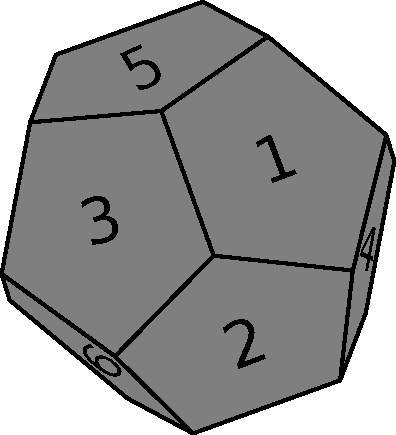
\includegraphics[width=1\linewidth]{sources/dice_rolls/images/3d_dices}
		\caption{Example of dice with $12$ faces.}
		\label{fig:dice_rolls:12faces_dice}
	 \end{subfigure}
	\hfill
	\begin{subfigure}[t]{0.25\textwidth}
		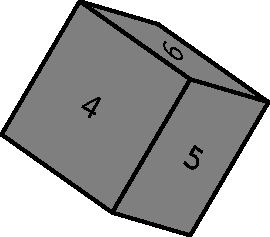
\includegraphics[width=1\linewidth]{sources/dice_rolls/images/cubic_dice}
		\caption{Example of common $6$ faces dice.}
		\label{fig:cycle_in_list:6faces_dice}
	 \end{subfigure}
	 \hfill
	 \begin{subfigure}[t]{0.25\textwidth}
		 \includegraphics[width=1\linewidth]{sources/dice_rolls/images/icosahedron_dice}
		 \caption{Example of dice with $20$ faces.}
		 \label{fig:cycle_in_list:20faces_dice}
	  \end{subfigure}
\end{figure}

\section{Discussion}
\label{dice_rolls:sec:discussion}
Let's start by noticing that the answer can be astronomically high but crucially that the number of
possible combinations of values resulting from rolling $d$ dices is even larger: if each dice has
$f$ faces, then we are looking at $f^d$ possible distinct roll outcomes! Therefore, a  brute-force
approach, where we go over each and every possible roll of the $d$ dices is completely out of the
picture given the constraints on the maximum number of of dices and faces we might get for input
unless you are willing to wait around \num{6e18} years \footnote{Even considering you implement this
algorithm so that it can run on the fastest supercomputer available today\cite{top500november2020},
which is capable of a staggering $\approx450$ \textbf{petaflop} operations per second, it would
still require $\frac{30^{30}}{10e15}$\si{\second} to run to completion. By that time humanity will
be long gone and the universe a dark and cold place.}.


This type of \textit{"counting"} questions are usually solved by using a dynamic programming
approach. In-fact this problem share a lot of similarities with the classical dynamic programming
\textit{Coin change} question we discussed in Chapter \ref{ch:coin_change}, to the point that you
could solve this problem using the solution to the other. If you are unfamiliar the solutions to the
\textit{Coin Change} problem you might want to refresh your memory before reading-on. We can
consider the problem treated in this chapter to be a proper specialization of the \textit{Coin
change} (Chapter \ref{ch:coin_change}) problem where the number of available coins is equal to $d$
and the denomination of the coins are $1,2,\ldots,f$: we have a coin of the same denomination as the
dice faces.


\subsection{Brute-force}
\label{dice_rolls:sec:bruteforce}
The brute-force approach will simply evaluate all possible outcomes of rolling $d$ dices and keep
track of how many yield a total sum of $t$. When dealing with this kind of tasks where you have to
enumerate things, recursion is usually the way to go, especially if the combination you are
generating can be defined recursively. In this specific case we can generate all combinations of
faces we can get from rolling $d$ dices by:
\begin{enumerate}
	\item first generating the combinations from rolling $d-1$ dices,
	\item create $f$ copies of them
	\item preprend $1$ to the items of the first copy
	\item preprend $2$ to the items of the second copy
	\item $\ldots$
	\item preprend $f$ to the items of the last copy
\end{enumerate}
The definition above is correct but not very useful in prectice as it requires to make many copies
of a potentially very large (exponentially) set of items. We will therefore use a different approach
that will still run in exponential time but can be used as a basis for developing a more efficient
DP solution.

We start by rolling the first dice; clearly for this die we have $f$ possible values we can get, but
once the value for this specific die is set, say we got the value $x$, we are left with $d-1$ dices
to roll still have to make up for $t-x$ with those $d-1$ dice in order to reach our target value
$t$. Once a die is rolled we are left with exactly the original problem on a smaller number of dice
and target value. This is why recursion is handy. The approach is easily defined in terms of
sub-problems. We can continue this recursive process until we reach one of the following cases:
\begin{enumerate}
	\item $d<0$ or $t<0$ the answer is $0$. There is no solution to the problem when the number of
	dices to use is negative or the target number is negative.
	\item $t=0$. We have reached the target value $t$. If we have used \textbf{all} dices then we
	have a solution, otherwise we do not. In other words:
	\begin{itemize}
		\item if $d=0$, we have used all $d$ dices and the sum is exactly equal to $t$. This is a
		valid combination. We have rolled $d$ dice and the sum of their faces is exactly equal to
		$t$.
		\item if $d>0$, we have not rolled all the dices, yet we have already reached our target
		value. If we continue to roll we will generate a combination with a total sum higher than
		$t$. This is not a good combination.
	\end{itemize}
\end{enumerate}
The idea above can be better expressed using the recurrence relation shown in Equation
\ref{eq:dice_rolls:dpformula} where $S(d,t,f)$ is the number of ways one can obtain a target value
$t$ by throwing $d$ dice. Notice that the third parameter never changes and thus, does not play a
dynamic role in the recurrence. It never changes. 

\begin{equation}
	S(d,t,f)=\begin{cases}
		 1 \: \: \text{ if } \: d=t=0 \\
		 0 \: \: \text{ if } \: d=0, \: t>0 \\ \\
		\sum_{1}^{\min(f,t)} S(d-1,t-j,f)  \:\: \text{ otherwise}
	 \end{cases}
	\label{eq:dice_rolls:dpformula}
\end{equation}

Listing \ref{list:dice_rolls:bruteforce} shows a possible implementation of such idea. Please note
that this code is remarkably similar to the brute-force solution for the Coin Change problem in
Chapter \ref{ch:coin_change}. Section
\ref{sec:min_difficulty_job_scheduler:generate_all_combination} also discuss the problem of
generating combinations, and the material discussed there can be adapted and applied here.
\lstinputlisting[language=c++, caption={Brute-force (enumerating all possible combinations) solution for the problem of counting the number of dice rolls summing up to a target number $t$.},label=list:dice_rolls:bruteforce]{sources/dice_rolls/dice_rolls_solution1.cpp}

The time and  space complexity of this approach are exponential and constant, respectively: The proof of
this fact can be derived from the solution of the following recurrence relation:
\begin{equation}
	S(d,t) = S(d-1,t-1) + S(d-1,t-2)
\label{eq:dice_rolls:dpformula}
\end{equation}
$S(d,t)$ is a recurrence relation expressing the number of invocation of the function 
\inline{num_rolls_to_target_bruteforce} 
for a given number of dice $d$ and target value $t$ when $f=2$. The resulting invocation tree is
complete and has height $h=t$ (assuming $d \leq t$, but the same reasoning can be applied in the
other case ). The cost of each node of the tree is $O(1)$. The number of nodes in such a tree is
exponential in its height. 

\subsection{Dynamic Programming - Recursive top-down}
\label{dice_rolls:sec:DP}
The brute-force solution we laid down in Section \ref{} can be however turned into a nice and
efficient one with the help of DP and in particular of memoization. As per many other problems
solvable with DP out there, Listing \ref{list:dice_rolls:bruteforce} can be turned into a much more
efficient solution by simply realizing that the same sub-problems are solved over and over again.
Imagine for instance the case where $f=5$. We might end up solving the sub-problem where $d=1$ and
$t=3$  from the sub-problem where $d=2$, $t=4$ (by rolling the face with $1$), or from the
sub-problem $d=2$, $t=5$ (by rolling the face with $2$).

However, the maximum number of different invokations for the function
\inline{num_rolls_to_target_bruteforce} is not larger than: $30\times 1000 = 30000$: the max number
of dice multipled  multiplied by the largest target value. The number of dice and the target value
are the only function parameters that vary during the execution. If we can somehow guarantee that no
duplicate work is done for a given $d$ and $t$, then we can get away with only $O(d\times t)$
function calls. When this happens we can simply store the result of intermediate problems into a
cache and use the values in the cache before trying to compute the answer (see Chapter
\ref{valid_parenthesis:sec:dp}). For instance consider what happens during the execution of the code
in Listing \ref{list:dice_rolls:bruteforce} for the following input:
\begin{itemize}
	\item $d = 3$
	\item $f = 6$
	\item $t = 12$
\end{itemize}

The function subproblem \inline{num_rolls_to_target_bruteforce(1,5,6)} solved $6$ times and the
subproblem \inline{num_rolls_to_target_bruteforce(1,4,6)} is solved $5$ times. If you are not
convinced draw the recursion tree, or add a print statement at the beginning of the function. All
these superfluous execution can be avoided if the result of each of the subproblem is stored into a
cache as shown in Listing \ref{list:dice_rolls:dp}. This implementation is an almost identical copy
of the brute-force solution with the addition of a cache. Note how \textbf{before} actually trying
to compute the answer we first look into the cache to see if we already did. If not, we solve the
problem and before returning the answer we \textbf{save} the result into the cache.
\lstinputlisting[language=c++, caption={Dynamic programming with memoization top-down recursive  solution for the problem of counting the number of dice rolls summing up to a target number $t$.},label=list:dice_rolls:dp]{sources/dice_rolls/dice_rolls_solution2.cpp}


\section{Dynamic programming - Iterative bottom-up}
\label{dice_rolls:sec:bottom}
Turning the top-down-up solution shown in Section \ref{} is relatively easy because the recursive
definition of the solution (Equation \ref{eq:dice_rolls:dpformula}) clearly show that you can
calculate the answer for a given number of dice $d$ and a target value $t$ if you have already
calculated the values for targets $t-1, t-2, \ldots, t-f$ and $d-1$. We also know how to easily
calculate the answer for all possible target values when $d=0$ and $d=1$ and from there we can apply
the reasoning above. 

This is exactly the strategy that Listing \ref{list:dice_rolls:dpbottomup} implements. We use a 2D
table $DP$ (initialized with zeros) with $d+1$ rows and $t+1$ columns where each cell $DP[i][j]$
correspond to the solution of a subproblem where $d=i$ and $t=j$. The first loop takes care of
filling the table with "known" values, for all sub-problems where $d=1$. If you only have a die with
$f$ faces, there is only one way you can achieve the target values $1,2,\ldots, f$ and no way to
obtain any higher values. The rest of the code fills the table one row at a time (one dice at a
time) by using the values of the previous row. 

\lstinputlisting[language=c++, caption={Dynamic programming bottom-up solution for the problem of counting the number of dice rolls summing up to a target number $t$.},label=list:dice_rolls:dpbottomup]{sources/dice_rolls/dice_rolls_solution3.cpp}

The time and space complexity of the code shown in Listing \ref{list:dice_rolls:dpbottomup}
are $\Theta(dtf)$ and $\Theta(dt)$, respectively. However the space complexity can be lowered easily
down  to $\Theta(t)$ because, as already mentioned, we only need space for two rows of the DP table:
one for the values of the current $d$ and one for the values at $d-1$. Listing
\ref{list:dice_rolls:dpbottomup} can be easily modified to add this optimization and we leave this
as an exercise for the reader.



